% lint-skip: 未完成ステータス（figure/table caption 未対応，人手チェック時に解消予定）
\documentclass[../../main.tex]{subfiles}
\begin{document}

\begin{flushright}
  \footnotesize\textit{【自動文字起こし・要確認】}
\end{flushright}

\noindent
{\bf [解答]} $A$ を原点，$B(2,0), C(0,2)$ とする $xy$ 平面で考える．又，$O(t,t)\ (0 < t)$ とおき題意の円を $T$ とおく．
\[
  T : (x-t)^2 + (y-t)^2 = 1
\]
\[
  BC : x+y = 2
\]

\begin{figure}[htb]
  \centering
  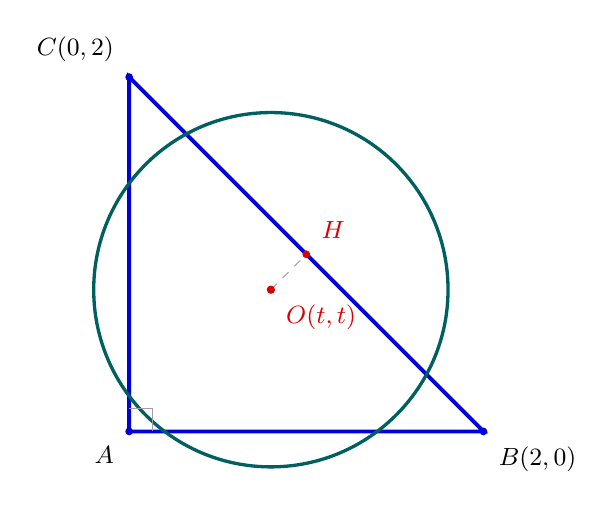
\begin{tikzpicture}[x=2.25cm, y=2.25cm, >=stealth,
    every node/.style={font=\small}]
    % Representative t=0.8 in the admissible range sqrt(2)/2 <= t < 1.
    \coordinate (A) at (0,0);
    \coordinate (B) at (2,0);
    \coordinate (C) at (0,2);
    \coordinate (O) at (0.8,0.8);
    \coordinate (H) at (1,1);
    \draw[line width=1.4pt, blue!85!black] (A) -- (B) -- (C) -- cycle;
    \draw[line width=1.2pt, teal!75!black] (O) circle[radius=1];
    \draw[dashed, gray!70] (O) -- (H);
    \draw[gray!75] (0,0.13) -- (0.13,0.13) -- (0.13,0);
    \foreach \P in {A,B,C} {\fill[blue!85!black] (\P) circle (1.4pt);}
    \fill[red!85!black] (O) circle (1.5pt);
    \fill[red!85!black] (H) circle (1.4pt);
    \node[below left=2pt] at (A) {$A$};
    \node[below right=2pt] at (B) {$B(2,0)$};
    \node[above left=2pt] at (C) {$C(0,2)$};
    \node[below right=2pt, red!85!black] at (O) {$O(t,t)$};
    \node[above right=2pt, red!85!black] at (H) {$H$};
  \end{tikzpicture}
  \caption{三角形 $ABC$ と中心 $O(t,t)$，半径1の円 $T$}
\end{figure}

\begin{enumerate}
  \item[(i)] $T$ と $x$ 軸の交点は $x^2 - 2tx + 2t^2 - 1 = 0$ の2実解

    $T$ と $y$ 軸の交点は $y^2 - 2ty + 2t^2 - 1 = 0$ の2実解

    $T$ と $BC$ の交点は $2x^2 - 4x + 2t^2 - 4t + 3 = 0$ の2実解

    だからこれらが $0 \le x \le 2, 0 \le y \le 2$ に2実解を持つ条件を考えて，

    \begin{align}
      &
      \begin{cases}
        \text{軸}: 0 < t < 2 \\
        \text{端}: 2t^2 - 1 \ge 0, \ 2t^2 - 4t + 3 \ge 0 \\
        \text{判}: t^2 - (2t^2 - 1) > 0
      \end{cases}
      \quad \wedge \quad
      \begin{cases}
        \text{軸}: 0 < 1 < 2 \\
        \text{端}: 2t^2 - 4t + 3 \ge 0, \ 2t^2 - 4t + 3 \ge 0 \\
        \text{判}: 4 - 2(2t^2 - 4t + 3) > 0
      \end{cases}
      \\
      &\iff
      \begin{cases}
        0 < t < 2 \\
        \dfrac{\sqrt{2}}{2} \le t < 1
      \end{cases}
      \quad \wedge \quad
      2 - \sqrt{2} < t < 2 + \sqrt{2} \\
      &\iff \dfrac{\sqrt{2}}{2} \le t < 1
    \end{align}
    よって，$x = 1/t$ だから，$1 \le x < \sqrt{2}$．

  \item[(ii)] (i)の時，$T$ の中心と $x, y$ 軸，$BC$ との距離は各々
    \[
      t, \quad t, \quad |\sqrt{2} - \sqrt{2}t|
    \]
    だから，$F(t)$ が右図斜線部の面積を表すことから，

    \begin{figure}[htb]
      \centering
      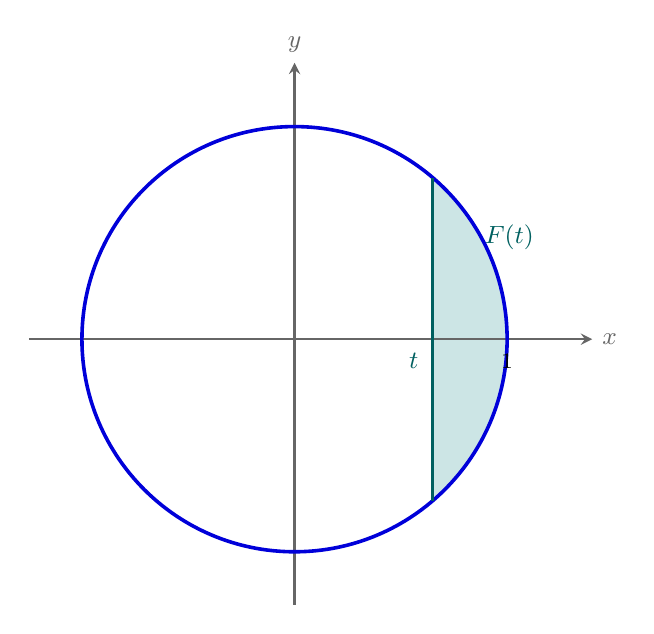
\begin{tikzpicture}[x=2.7cm, y=2.7cm, >=stealth,
        every node/.style={font=\small}]
        % A sample cut 0<t<1; the shaded circular cap has area F(t).
        \pgfmathsetmacro{\cut}{0.65}
        \begin{scope}
          \clip (0,0) circle[radius=1];
          \fill[teal!20] (\cut,-1.1) rectangle (1.1,1.1);
        \end{scope}
        \draw[->, thick, gray!80!black] (-1.25,0) -- (1.4,0) node[right] {$x$};
        \draw[->, thick, gray!80!black] (0,-1.25) -- (0,1.3) node[above] {$y$};
        \draw[line width=1.3pt, blue!85!black] (0,0) circle[radius=1];
        \draw[line width=1.1pt, teal!75!black] (\cut,{-sqrt(1-\cut*\cut)})
        -- (\cut,{sqrt(1-\cut*\cut)});
        \node[below left=4pt, teal!75!black, fill=white, inner sep=1pt]
        at (\cut,0) {$t$};
        \node[right=3pt, teal!75!black] at (0.81,0.48) {$F(t)$};
        \node[below=2pt, font=\footnotesize] at (1,0) {$1$};
      \end{tikzpicture}
      \caption{単位円で直線 $x=t$ の右側にある円弓形の面積 $F(t)$}
    \end{figure}

    \[
      S = \pi - 2F\left(\dfrac{1}{x}\right) - F(\sqrt{2} - x)
    \]

  \item[(iii)] (ii)から
    \begin{align}
      \dfrac{dS}{dx} &= +4 \sqrt{1 - \dfrac{1}{x^2}} \cdot \dfrac{1}{x^2} - 2\sqrt{1 - (\sqrt{2}-x)^2} \\
      &= 2 \left[ \sqrt{2 - x^2} - \sqrt{1 - (\sqrt{2}-x)^2} \right] \\
      &= 2 \dfrac{-2\sqrt{2}x + 3}{\sqrt{2-x^2} + \sqrt{1 - (\sqrt{2}-x)^2}}
    \end{align}
    から下表を得る．

    \begin{center}
      \begin{table}[htb]
        \centering
        \begin{tabular}{c|c|c|c|c|c}
          $x$ & $1$ & $\dots$ & $\dfrac{3}{4}\sqrt{2}$ & $\dots$ & $\sqrt{2}$ \\ \hline
          $S'$ & & $+$ & $0$ & $-$ & \\ \hline
          $S$ & & $\nearrow$ & & $\searrow$ &
        \end{tabular}
      \end{table}
    \end{center}

    よって，$x = \dfrac{3}{4}\sqrt{2}$ で $S$ は最大．
\end{enumerate}

\end{document}
